\chapter{Development tools}
\label{sec:development-tools}

For experimental work and implementation purposes we used the Kinect SDK in combination with EMGU (C\#) and OpenNI combined with OpenCV (C++). The Kinect SDK and OpenNI were used to capture colour and depth images from the Kinect sensor. The initial preliminary work for basic foreground extraction was done using the computer vision library EMGU and the Kinect SDK. The majority of the experimental work that was done later on, was implemented in OpenCV because it provided more features, more openness and better flexibility in programming.

\section{OpenCV}
\label{sec:opencv}

\textit{OpenCV} is an open source library consisting of computer vision algorithms, and was originally developed by \textit{Intel} and is now supported by \textit{Willow Garage} and \textit{Itseez}. OpenCV consists of libraries mainly for C/C++ development and interfaces are also provided for Python, Java and Matlab. EMGU is a wrapper of OpenCV libraries and is used for .Net development. Part of the OpenCV framework are CUDA and OpenCL based GPU interfaces. The basic structure of OpenCV is the core module that contains methods for data structure definition and matrix manipulation, the image processing module that includes various image processing algorithms, the interface module that offers image and video loading and presenting capabilities, the feature description and detection module, the machine learning module and other computer vision related modules that are useful for application or experimental development.

\section{Kinect}
\label{sec:kinect}

The Kinect sensor is a consumer grade imaging device developed by \textit{Microsoft} in 2010 to be used as a natural interaction medium for computer game environments, with original development by Israeli company \textit{PrimeSence}. Its low cost, though, along with its range sensing capabilities has attracted the attention of researchers and computer vision enthusiasts. The Kinect sensor can produce depth and colour streams simultaneously at a frame rate of 30 fps with resolutions 640X480. The colour stream is also scaled to 1280X960 resolution at 15 fps. The sensor consists of an infrared laser emitter, an infrared camera and an RGB camera. The depth is measured by a triangulation process, where the laser emits a beam that is split into multiple beams by a diffraction grating to create a constant pattern of speckles projected onto the scene \cite{kinectaccuracy}. The produced pattern is captured by the infrared camera and correlated against a reference pattern to estimate depth. This method for extracting depth information is also known as \textit{structured light scanning} \cite{kinectaccuracy}. The depth measurement is in millimetres and depth sensing ranges from 400mm to 8000mm (Figure \ref{fig:depth-dist}).

\section{Kinect SDK and OpenNI}
\label{sec:openni}

The original Kinect was released for the Xbox 360 in 2010 and a Windows version for development purposes was released later on along with the Kinect SDK in 2012. The Kinect SDK has a core module called Natural User Interface that handles colour and depth streams, player and skeletal tracking and audio streams, a module for gesture recognition, the Kinect Fusion module that deals with 3D reconstruction, a face tracking module, a back removal module and a module for web application development. The Natural User Interface module handles the depth stream in different resolutions and formats. As mentioned previously, the depth measures from 400mm to 8000mm but the recommended values are the ones between 800mm and 4000mm; distances further than 4000mm are considered too far and distances closer than 800mm are considered too near (Figure \ref{fig:depth-dist}). Flags can be set for the desired depth stream distances to be used.
\par
\textit{OpenNI} is a framework that contains open source drivers and APIs that provide tools for gesture recognition, body motion tracking and other natural interaction interfaces. It is supported mainly by PrimeSence and Asus, that have developed their own range sensing devices, and Willow Garage, a computer vision and robotics research centre. PrimeSence has been acquired by Apple in 2013 and subsequently in April 2014 OpenNI website was shut down. Forks of older versions of the framework can still be found online. Unfortunately the components of OpenNI are limited to basic stream acquisition, skeletal and hand tracking and some other features, since the more advanced features were part of Nite that was developed by Primesence and now is not available.

\begin{figure}[t!]
\centering
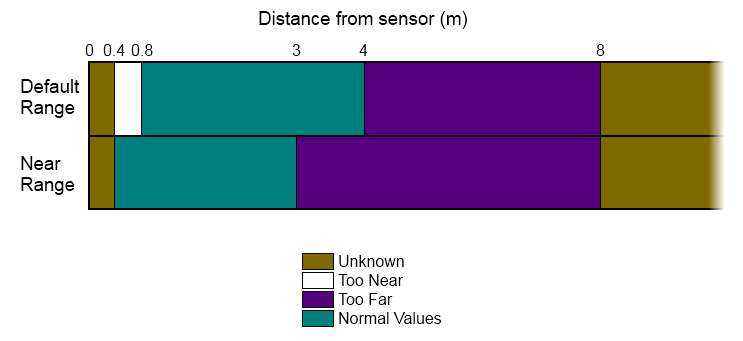
\includegraphics[width=1\columnwidth]{Chapter3/3/depth_dist.png}
\caption[Depth stream distances.]{The Kinect SDK handles the depth stream by separating the distances in to categories that the developer can choose from depending on the application.}
\label{fig:depth-dist}
\end{figure}